% Build with XeLaTeX (Indic scripts): xelatex main && bibtex main && xelatex main && xelatex main
% Overleaf: Menu > Compiler > XeLaTeX.  acl.sty and acl_natbib.bst are the unmodified official ACL style files.
\PassOptionsToPackage{table}{xcolor}   % row shading in tables (acl.sty loads xcolor)
\documentclass[11pt]{article}

% `preprint' is the official ACL option that shows author names and affiliations (the demo track is single-blind).
\usepackage[preprint]{acl}
\usepackage{microtype}
\usepackage[english,bidi=default]{babel}
\babelfont{rm}[SmallCapsFeatures={Letters=SmallCaps}]{TeXGyreTermesX}
\usepackage{fontspec}
% Noto Sans Devanagari / Gujarati are bundled in fonts/ (SIL OFL 1.1), so the build needs no system fonts for Indic text.
\newfontfamily\hifont[Path=fonts/,Extension=.ttf,UprightFont=NotoSansDevanagari-Regular,BoldFont=NotoSansDevanagari-Bold,Script=Devanagari]{NotoSansDevanagari}
\newfontfamily\gufont[Path=fonts/,Extension=.ttf,UprightFont=NotoSansGujarati-Regular,BoldFont=NotoSansGujarati-Bold,Script=Gujarati]{NotoSansGujarati}
% Native-script text is typeset upright in a locally scoped font. A PDF ActualText span keeps the source order of the Unicode string,
% so that copying text from the PDF returns the authored word (without it, the pre-base vowel sign of Hindi 'chahie' is extracted out of order).
% \pdfstringdef (hyperref) builds a UTF-16 PDF string; the span is emitted only under XeTeX (Overleaf: XeLaTeX; Tectonic).
\newcommand{\aacnative}[2]{\leavevmode\begingroup
  \ifdefined\XeTeXversion
    \pdfstringdef\aacactual{#2}%
    \special{pdf:literal direct /Span <</ActualText (\aacactual)>> BDC}%
  \fi
  {#1\upshape #2}%
  \ifdefined\XeTeXversion\special{pdf:literal direct EMC}\fi
  \endgroup}
\DeclareRobustCommand{\hi}[1]{\aacnative{\hifont}{#1}}   % Hindi and Marathi (Devanagari)
\DeclareRobustCommand{\gu}[1]{\aacnative{\gufont}{#1}}   % Gujarati
\usepackage{booktabs,graphicx,amsmath,amssymb,array,multirow,xcolor,colortbl,enumitem,float}
% Palette (also legible in grayscale because every colored span is accompanied by a verdict mark or a word):
% blue = selected concept kept, green = successful sentence, red = unwanted act, added or third-person content.
\definecolor{exblue}{HTML}{155B8A}\definecolor{exgreen}{HTML}{17674A}\definecolor{exred}{HTML}{AC252B}
\definecolor{headtint}{HTML}{E9F0F6}\definecolor{rowtint}{HTML}{F6F8FA}
\newcommand{\sel}[1]{\textcolor{exblue}{#1}}
\newcommand{\kept}[1]{\textcolor{exgreen}{#1}}
\newcommand{\bad}[1]{\textcolor{exred}{#1}}
\newcommand{\okmark}{\textcolor{exgreen}{\ensuremath{\checkmark}}}
\newcommand{\failmark}[1]{\textcolor{exred}{\ensuremath{\times}\textsuperscript{\scriptsize #1}}}
\newcommand{\routem}{{\scriptsize\emph{model}}}      % route tag: accepted model output
\newcommand{\routet}{{\scriptsize\emph{template}}}   % route tag: template floor
\makeatletter\pdfstringdefDisableCommands{\let\sel\@firstofone\let\kept\@firstofone\let\bad\@firstofone}\makeatother
\newcommand{\lang}[1]{\textbf{\emph{#1}}}      % language label: bold italic, apart from the upright native script
\newcommand{\llm}[1]{\mbox{\textsc{#1}}}              % model names: small capitals at the body size
\newcommand{\qwen}{\llm{Qwen2.5-0.5B-Instruct}}
\newcommand{\indicf}{\llm{IndicF5}}
\newcommand{\vocos}{\llm{Vocos}}
\newcommand{\flant}{\llm{Flan-T5-small}}
\newcommand{\utmos}{\llm{UTMOS22}}
\newcommand{\nisqa}{\llm{NISQA}}
\newcommand{\mmstts}{\llm{MMS-TTS}}
\newcommand{\gloss}[1]{\emph{``#1''}}           % English gloss in italics
\setlist{nosep,leftmargin=*}
\hyphenation{Table Tables Figure Appendix Section}   % keep reference words whole
\setcounter{topnumber}{3}\setcounter{bottomnumber}{2}\setcounter{totalnumber}{5}\setcounter{dbltopnumber}{3}
\renewcommand{\topfraction}{0.9}\renewcommand{\bottomfraction}{0.8}\renewcommand{\textfraction}{0.08}
\renewcommand{\floatpagefraction}{0.75}\renewcommand{\dblfloatpagefraction}{0.75}
\newcolumntype{L}[1]{>{\raggedright\arraybackslash}p{#1}}

\newcommand{\sys}{Indic AAC Studio}
\newcommand{\nstated}{\textit{n.s.}}
\newcommand{\cn}[1]{\raisebox{.15ex}{\textcircled{\scriptsize #1}}}   % numbered callout used in Figure 2
% Release location of the reviewer package (source, fixtures, scorer, raw outputs, screencast): AUTHORS MUST SET THIS to a public (or anonymized) URL before submission.
\newcommand{\demourl}{\url{https://github.com/speechforge/AAC_System}}
% Code license named in the Availability section: AUTHORS MUST CONFIRM and add the matching license file to the release.
\newcommand{\codelicense}{Apache License 2.0}
% Required concept instances in the primary set: the denominator of the Kept column of Table 2.
\newcommand{\NConc}{215}

% generated/ holds numbers and tables produced from the frozen evaluation files; v3 relabeled and re-captioned them by hand and corrected one printed cell (Hindi bigram hit@1, 24.1 to 24.0, from 586/2437 = 24.05%).
% Numbers typed in the sections (intervals, gate precision, repair counts, latencies) are rechecked by the scripts in after_the_proof_reading_final_version/qa_scripts.
% AUTO-GENERATED by eval/make_tex.py from eval/results/*.json -- do not edit
\newcommand{\NScen}{184}
\newcommand{\NScenCM}{8}
\newcommand{\NOverlap}{9}
\newcommand{\NPrimEN}{46}
\newcommand{\NAllEN}{46}
\newcommand{\NPrimHI}{45}
\newcommand{\NAllHI}{46}
\newcommand{\NPrimGU}{42}
\newcommand{\NAllGU}{46}
\newcommand{\NPrimMR}{42}
\newcommand{\NAllMR}{46}
\newcommand{\NPrimAll}{175}
\newcommand{\PDNEN}{\mbox{+43\,pp [+28, +59]}}
\newcommand{\CDNEN}{22/46\,vs\,2/46}
\newcommand{\PDNHI}{\mbox{+67\,pp [+53, +80]}}
\newcommand{\CDNHI}{31/45\,vs\,1/45}
\newcommand{\PDNGU}{\mbox{+40\,pp [+24, +57]}}
\newcommand{\CDNGU}{21/42\,vs\,4/42}
\newcommand{\PDNMR}{\mbox{+52\,pp [+36, +69]}}
\newcommand{\CDNMR}{23/42\,vs\,1/42}
\newcommand{\PDTEN}{\mbox{\ensuremath{-}24\,pp [\ensuremath{-}37, \ensuremath{-}13]}}
\newcommand{\CDTEN}{22/46\,vs\,33/46}
\newcommand{\PDTHI}{\mbox{+0\,pp [+0, +0]}}
\newcommand{\CDTHI}{31/45\,vs\,31/45}
\newcommand{\PDTGU}{\mbox{\ensuremath{-}14\,pp [\ensuremath{-}26, \ensuremath{-}5]}}
\newcommand{\CDTGU}{21/42\,vs\,27/42}
\newcommand{\PDTMR}{\mbox{\ensuremath{-}10\,pp [\ensuremath{-}21, +0]}}
\newcommand{\CDTMR}{23/42\,vs\,27/42}
\newcommand{\PDPEN}{\mbox{+41\,pp [+26, +57]}}
\newcommand{\CDPEN}{22/46\,vs\,3/46}
\newcommand{\PDPHI}{\mbox{+16\,pp [+7, +27]}}
\newcommand{\CDPHI}{31/45\,vs\,24/45}
\newcommand{\PDPGU}{\mbox{+2\,pp [+0, +7]}}
\newcommand{\CDPGU}{21/42\,vs\,20/42}
\newcommand{\PDPMR}{\mbox{+12\,pp [+2, +24]}}
\newcommand{\CDPMR}{23/42\,vs\,18/42}
\newcommand{\PSUEN}{\mbox{+24\,pp [+13, +37]}}
\newcommand{\CSUEN}{33/46\,vs\,22/46}
\newcommand{\PSUHI}{\mbox{+22\,pp [+11, +36]}}
\newcommand{\CSUHI}{41/45\,vs\,31/45}
\newcommand{\PSUGU}{\mbox{+12\,pp [+2, +21]}}
\newcommand{\CSUGU}{26/42\,vs\,21/42}
\newcommand{\PSUMR}{\mbox{+21\,pp [+7, +36]}}
\newcommand{\CSUMR}{32/42\,vs\,23/42}
\newcommand{\PSTEN}{\mbox{\ensuremath{-}28\,pp [\ensuremath{-}41, \ensuremath{-}15]}}
\newcommand{\CSTEN}{33/46\,vs\,46/46}
\newcommand{\PSTHI}{\mbox{\ensuremath{-}9\,pp [\ensuremath{-}18, \ensuremath{-}2]}}
\newcommand{\CSTHI}{41/45\,vs\,45/45}
\newcommand{\PSTGU}{\mbox{\ensuremath{-}19\,pp [\ensuremath{-}31, \ensuremath{-}7]}}
\newcommand{\CSTGU}{26/42\,vs\,34/42}
\newcommand{\PSTMR}{\mbox{\ensuremath{-}24\,pp [\ensuremath{-}38, \ensuremath{-}12]}}
\newcommand{\CSTMR}{32/42\,vs\,42/42}
\newcommand{\PSPEN}{\mbox{+61\,pp [+46, +74]}}
\newcommand{\CSPEN}{33/46\,vs\,5/46}
\newcommand{\PSPHI}{\mbox{+33\,pp [+20, +47]}}
\newcommand{\CSPHI}{41/45\,vs\,26/45}
\newcommand{\PSPGU}{\mbox{+24\,pp [+12, +38]}}
\newcommand{\CSPGU}{26/42\,vs\,16/42}
\newcommand{\PSPMR}{\mbox{+19\,pp [+7, +31]}}
\newcommand{\CSPMR}{32/42\,vs\,24/42}
\newcommand{\PLLEN}{\mbox{\ensuremath{-}4\,pp [\ensuremath{-}11, +0]}}
\newcommand{\CLLEN}{1/46\,vs\,3/46}
\newcommand{\PLLHI}{\mbox{+0\,pp [+0, +0]}}
\newcommand{\CLLHI}{24/45\,vs\,24/45}
\newcommand{\PLLGU}{\mbox{+0\,pp [+0, +0]}}
\newcommand{\CLLGU}{20/42\,vs\,20/42}
\newcommand{\PLLMR}{\mbox{+0\,pp [+0, +0]}}
\newcommand{\CLLMR}{18/42\,vs\,18/42}
\newcommand{\FBUAll}{61/184}
\newcommand{\FBUEN}{30/46}
\newcommand{\FBpctUEN}{65\%}
\newcommand{\ErrUEN}{0}
\newcommand{\FBUHI}{8/46}
\newcommand{\FBpctUHI}{17\%}
\newcommand{\ErrUHI}{0}
\newcommand{\FBUGU}{6/46}
\newcommand{\FBpctUGU}{13\%}
\newcommand{\ErrUGU}{0}
\newcommand{\FBUMR}{17/46}
\newcommand{\FBpctUMR}{37\%}
\newcommand{\ErrUMR}{0}
\newcommand{\FBSAll}{67/184}
\newcommand{\FBSEN}{28/46}
\newcommand{\FBpctSEN}{61\%}
\newcommand{\ErrSEN}{0}
\newcommand{\FBSHI}{15/46}
\newcommand{\FBpctSHI}{33\%}
\newcommand{\ErrSHI}{0}
\newcommand{\FBSGU}{16/46}
\newcommand{\FBpctSGU}{35\%}
\newcommand{\ErrSGU}{0}
\newcommand{\FBSMR}{8/46}
\newcommand{\FBpctSMR}{17\%}
\newcommand{\ErrSMR}{0}
\newcommand{\LatAllEN}{11.75\,s (p90 12.75, n=69)}
\newcommand{\LatAcceptedEN}{6.05\,s (p90 6.23, n=22)}
\newcommand{\LatFallbackEN}{12.04\,s (p90 12.81, n=47)}
\newcommand{\LatAllHI}{9.97\,s (p90 18.85, n=70)}
\newcommand{\LatAcceptedHI}{9.75\,s (p90 10.08, n=52)}
\newcommand{\LatFallbackHI}{18.76\,s (p90 20.12, n=18)}
\newcommand{\LatAllGU}{7.5\,s (p90 14.77, n=72)}
\newcommand{\LatAcceptedGU}{7.45\,s (p90 7.58, n=51)}
\newcommand{\LatFallbackGU}{14.73\,s (p90 15.06, n=21)}
\newcommand{\LatAllMR}{6.58\,s (p90 13.05, n=72)}
\newcommand{\LatAcceptedMR}{6.51\,s (p90 7.06, n=49)}
\newcommand{\LatFallbackMR}{13.0\,s (p90 13.81, n=23)}
\newcommand{\LatMedAccEN}{6.05}
\newcommand{\LatMedFbEN}{12.04}
\newcommand{\LatMedAccHI}{9.75}
\newcommand{\LatMedFbHI}{18.76}
\newcommand{\LatMedAccGU}{7.45}
\newcommand{\LatMedFbGU}{14.73}
\newcommand{\LatMedAccMR}{6.51}
\newcommand{\LatMedFbMR}{13.0}
\newcommand{\LatFbMin}{12.04}
\newcommand{\LatFbMax}{18.76}
\newcommand{\NUniqueReq}{283}
\newcommand{\StageLlmOne}{1.87}
\newcommand{\StageLlmTwo}{0.0}
\newcommand{\StageLlmThree}{4.63}
\newcommand{\StageSem}{0.0}
\newcommand{\StageTts}{0.0}
\newcommand{\StageTotal}{9.46}
\newcommand{\PredENOneInf}{17.2}
\newcommand{\PredENOneTri}{16.0}
\newcommand{\PredENFiveInf}{33.4}
\newcommand{\PredENFiveTri}{32.8}
\newcommand{\PredDENOneTri}{\mbox{+1.1\,pp [+0.5, +1.8]}}
\newcommand{\PredDENFiveTri}{\mbox{+0.6\,pp [+0.0, +1.2]}}
\newcommand{\PredDENMrrTri}{\mbox{+0.007 [+0.002, +0.011]}}
\newcommand{\PredDENOneBi}{\mbox{+3.6\,pp [+2.3, +5.0]}}
\newcommand{\PredDENFiveBi}{\mbox{+3.9\,pp [+2.7, +5.1]}}
\newcommand{\PredDENMrrBi}{\mbox{+0.036 [+0.025, +0.049]}}
\newcommand{\PredDENOneUni}{\mbox{+13.5\,pp [+11.4, +15.7]}}
\newcommand{\PredDENFiveUni}{\mbox{+21.8\,pp [+19.0, +24.8]}}
\newcommand{\PredDENMrrUni}{\mbox{+0.171 [+0.148, +0.197]}}
\newcommand{\PredNEN}{2220}
\newcommand{\PredClustersEN}{60}
\newcommand{\PredOOVEN}{7.5\%}
\newcommand{\PredHIOneInf}{27.0}
\newcommand{\PredHIOneTri}{25.9}
\newcommand{\PredHIFiveInf}{44.1}
\newcommand{\PredHIFiveTri}{44.0}
\newcommand{\PredDHIOneTri}{\mbox{+1.2\,pp [+0.5, +1.9]}}
\newcommand{\PredDHIFiveTri}{\mbox{+0.1\,pp [\ensuremath{-}0.3, +0.4]}}
\newcommand{\PredDHIMrrTri}{\mbox{+0.008 [+0.004, +0.013]}}
\newcommand{\PredDHIOneBi}{\mbox{+3.0\,pp [+1.8, +4.3]}}
\newcommand{\PredDHIFiveBi}{\mbox{+1.0\,pp [+0.1, +1.9]}}
\newcommand{\PredDHIMrrBi}{\mbox{+0.023 [+0.014, +0.032]}}
\newcommand{\PredDHIOneUni}{\mbox{+20.6\,pp [+18.4, +23.0]}}
\newcommand{\PredDHIFiveUni}{\mbox{+29.5\,pp [+26.8, +32.4]}}
\newcommand{\PredDHIMrrUni}{\mbox{+0.243 [+0.220, +0.267]}}
\newcommand{\PredNHI}{2437}
\newcommand{\PredClustersHI}{60}
\newcommand{\PredOOVHI}{5.5\%}
\newcommand{\UIFalseNeg}{3}
\newcommand{\UISingle}{276}
\newcommand{\UIFeelReq}{27}
\newcommand{\GateAccU}{116}
\newcommand{\GateAccOkU}{57}
\newcommand{\GateAccPctU}{49\%}
\newcommand{\GateFbU}{59}
\newcommand{\GateFbOkU}{40}
\newcommand{\GateFbPctU}{68\%}
\newcommand{\GateAccS}{108}
\newcommand{\GateAccOkS}{71}
\newcommand{\GateAccPctS}{66\%}
\newcommand{\GateFbS}{67}
\newcommand{\GateFbOkS}{61}
\newcommand{\GateFbPctS}{91\%}
\newcommand{\CMSuccNaive}{0/8}
\newcommand{\CMSuccPre}{0/8}
\newcommand{\CMSuccDepU}{4/8}
\newcommand{\CMSuccDepS}{5/8}
\newcommand{\CMSuccTmplU}{6/8}
\newcommand{\CMSuccTmplS}{8/8}
\newcommand{\ActWrongUEN}{12/46}
\newcommand{\SuccEffUEN}{22/46}
\newcommand{\ActWrongSEN}{2/46}
\newcommand{\SuccEffSEN}{33/46}
\newcommand{\ActWrongUHI}{14/45}
\newcommand{\SuccEffUHI}{31/45}
\newcommand{\ActWrongSHI}{4/45}
\newcommand{\SuccEffSHI}{41/45}
\newcommand{\ActWrongUGU}{11/42}
\newcommand{\SuccEffUGU}{21/42}
\newcommand{\ActWrongSGU}{2/42}
\newcommand{\SuccEffSGU}{26/42}
\newcommand{\ActWrongUMR}{17/42}
\newcommand{\SuccEffUMR}{23/42}
\newcommand{\ActWrongSMR}{9/42}
\newcommand{\SuccEffSMR}{32/42}
\newcommand{\GutHitOne}{6.7}
\newcommand{\HiHmmHitOne}{24.5}
\newcommand{\CPzeroPol}{2.1\%}
\newcommand{\CPallConcept}{98.3\%}
\newcommand{\SuccNaive}{8/175}
\newcommand{\SuccPctNaive}{5\%}
\newcommand{\KeptNaive}{199/215}
\newcommand{\KeptPctNaive}{93\%}
\newcommand{\PolErrNaive}{2/175}
\newcommand{\ActWrongNaive}{3/175}
\newcommand{\AddedNaive}{7/175}
\newcommand{\OffNaive}{16/175}
\newcommand{\SuccPre}{65/175}
\newcommand{\SuccPctPre}{37\%}
\newcommand{\KeptPre}{175/215}
\newcommand{\KeptPctPre}{81\%}
\newcommand{\PolErrPre}{2/175}
\newcommand{\ActWrongPre}{54/175}
\newcommand{\AddedPre}{25/175}
\newcommand{\OffPre}{19/175}
\newcommand{\SuccDepU}{97/175}
\newcommand{\SuccPctDepU}{55\%}
\newcommand{\KeptDepU}{215/215}
\newcommand{\KeptPctDepU}{100\%}
\newcommand{\PolErrDepU}{0/175}
\newcommand{\ActWrongDepU}{54/175}
\newcommand{\AddedDepU}{4/175}
\newcommand{\OffDepU}{10/175}
\newcommand{\SuccDepS}{132/175}
\newcommand{\SuccPctDepS}{75\%}
\newcommand{\KeptDepS}{215/215}
\newcommand{\KeptPctDepS}{100\%}
\newcommand{\PolErrDepS}{0/175}
\newcommand{\ActWrongDepS}{17/175}
\newcommand{\AddedDepS}{3/175}
\newcommand{\OffDepS}{9/175}
\newcommand{\SuccTmplS}{167/175}
\newcommand{\SuccPctTmplS}{95\%}
\newcommand{\KeptTmplS}{215/215}
\newcommand{\KeptPctTmplS}{100\%}
\newcommand{\PolErrTmplS}{0/175}
\newcommand{\ActWrongTmplS}{0/175}
\newcommand{\AddedTmplS}{0/175}
\newcommand{\OffTmplS}{0/175}
\newcommand{\SuccTmplU}{118/175}
\newcommand{\SuccPctTmplU}{67\%}
\newcommand{\KeptTmplU}{215/215}
\newcommand{\KeptPctTmplU}{100\%}
\newcommand{\PolErrTmplU}{0/175}
\newcommand{\ActWrongTmplU}{57/175}
\newcommand{\AddedTmplU}{0/175}
\newcommand{\OffTmplU}{0/175}
\newcommand{\SuccLit}{0/175}
\newcommand{\SuccPctLit}{0\%}
\newcommand{\KeptLit}{215/215}
\newcommand{\KeptPctLit}{100\%}
\newcommand{\PolErrLit}{0/175}
\newcommand{\ActWrongLit}{0/175}
\newcommand{\AddedLit}{0/175}
\newcommand{\OffLit}{0/175}
\newcommand{\RefARules}{384/384}
\newcommand{\RefARulesPct}{100.0\%}
\newcommand{\RefAModel}{378/384}
\newcommand{\RefAModelPct}{98.4\%}
\newcommand{\RefAHybrid}{384/384}
\newcommand{\RefAHybridPct}{100.0\%}
\newcommand{\RefARaw}{0/384}
\newcommand{\RefARawPct}{0.0\%}
\newcommand{\RefALat}{31.8}
\newcommand{\RefFRules}{384/384}
\newcommand{\RefFRulesPct}{100.0\%}
\newcommand{\RefFModel}{379/384}
\newcommand{\RefFModelPct}{98.7\%}
\newcommand{\RefFHybrid}{384/384}
\newcommand{\RefFHybridPct}{100.0\%}
\newcommand{\RefFRaw}{0/384}
\newcommand{\RefFRawPct}{0.0\%}
\newcommand{\RefFLat}{32.2}
\newcommand{\IGSent}{15{,}505}
\newcommand{\IGTok}{112{,}875}
\newcommand{\IGDepth}{181}
\newcommand{\OffReady}{10.2}
\newcommand{\OffFirstEn}{13.94}
\newcommand{\OffHi}{10.1}
\newcommand{\NSymbols}{69}
\newcommand{\NCategories}{9}

% generated by make_tables.py from eval/results/*.json and scored.csv
\newcommand{\XPreSSucc}{71/175}
\newcommand{\XPreSSuccPct}{41\%}
\newcommand{\XPreSKept}{185/215}
\newcommand{\XPreSKeptPct}{86\%}
\newcommand{\XPreSPol}{36/175}
\newcommand{\XPreSWrong}{30/175}
\newcommand{\XPreSNoAct}{44/175}
\newcommand{\XPreSAdded}{21/175}
\newcommand{\XPreSOff}{17/175}
\newcommand{\XPreUSucc}{65/175}
\newcommand{\XPreUSuccPct}{37\%}
\newcommand{\XPreUKept}{175/215}
\newcommand{\XPreUKeptPct}{81\%}
\newcommand{\XPreUPol}{2/175}
\newcommand{\XPreUWrong}{54/175}
\newcommand{\XPreUNoAct}{33/175}
\newcommand{\XPreUAdded}{25/175}
\newcommand{\XPreUOff}{19/175}
\newcommand{\XDepSSucc}{132/175}
\newcommand{\XDepSSuccPct}{75\%}
\newcommand{\XDepSKept}{215/215}
\newcommand{\XDepSKeptPct}{100\%}
\newcommand{\XDepSPol}{0/175}
\newcommand{\XDepSWrong}{17/175}
\newcommand{\XDepSNoAct}{24/175}
\newcommand{\XDepSAdded}{3/175}
\newcommand{\XDepSOff}{9/175}
\newcommand{\XDepUSucc}{97/175}
\newcommand{\XDepUSuccPct}{55\%}
\newcommand{\XDepUKept}{215/215}
\newcommand{\XDepUKeptPct}{100\%}
\newcommand{\XDepUPol}{0/175}
\newcommand{\XDepUWrong}{54/175}
\newcommand{\XDepUNoAct}{21/175}
\newcommand{\XDepUAdded}{4/175}
\newcommand{\XDepUOff}{10/175}
\newcommand{\XTmplSSucc}{167/175}
\newcommand{\XTmplSSuccPct}{95\%}
\newcommand{\XTmplSKept}{215/215}
\newcommand{\XTmplSKeptPct}{100\%}
\newcommand{\XTmplSPol}{0/175}
\newcommand{\XTmplSWrong}{0/175}
\newcommand{\XTmplSNoAct}{8/175}
\newcommand{\XTmplSAdded}{0/175}
\newcommand{\XTmplSOff}{0/175}
\newcommand{\XTmplUSucc}{118/175}
\newcommand{\XTmplUSuccPct}{67\%}
\newcommand{\XTmplUKept}{215/215}
\newcommand{\XTmplUKeptPct}{100\%}
\newcommand{\XTmplUPol}{0/175}
\newcommand{\XTmplUWrong}{57/175}
\newcommand{\XTmplUNoAct}{0/175}
\newcommand{\XTmplUAdded}{0/175}
\newcommand{\XTmplUOff}{0/175}
\newcommand{\XNaiveSucc}{8/175}
\newcommand{\XNaiveSuccPct}{5\%}
\newcommand{\XNaiveKept}{199/215}
\newcommand{\XNaiveKeptPct}{93\%}
\newcommand{\XNaivePol}{2/175}
\newcommand{\XNaiveWrong}{3/175}
\newcommand{\XNaiveNoAct}{163/175}
\newcommand{\XNaiveAdded}{7/175}
\newcommand{\XNaiveOff}{16/175}
\newcommand{\XPolDropPreS}{35}
\newcommand{\XPolSpurPreS}{1}
\newcommand{\XGateAccU}{116}
\newcommand{\XGateAccPctU}{66\%}
\newcommand{\XGateFbU}{59}
\newcommand{\XGateFbPctU}{34\%}
\newcommand{\XGateOkU}{57/116}
\newcommand{\XGateOkPctU}{49\%}
\newcommand{\XFbOkU}{40/59}
\newcommand{\XFbOkPctU}{68\%}
\newcommand{\XGateAccS}{108}
\newcommand{\XGateAccPctS}{62\%}
\newcommand{\XGateFbS}{67}
\newcommand{\XGateFbPctS}{38\%}
\newcommand{\XGateOkS}{71/108}
\newcommand{\XGateOkPctS}{66\%}
\newcommand{\XFbOkS}{61/67}
\newcommand{\XFbOkPctS}{91\%}

% AUTO-GENERATED by mos_eval/make_mos_table.py from mos_eval/mos_scores.csv
\newcommand{\MosToneU}{1.5}
\newcommand{\MosToneN}{1.1}
\newcommand{\MosRefULo}{2.7}
\newcommand{\MosRefUHi}{4.3}
\newcommand{\MosStandULo}{3.3}
\newcommand{\MosStandUHi}{4.0}
\newcommand{\MosStandNLo}{3.5}
\newcommand{\MosStandNHi}{4.9}
\newcommand{\MosNStand}{175}
\newcommand{\MosNRef}{8}
\newcommand{\MosCorr}{0.47}


\title{Indic AAC Studio: Concept-Gated Symbol-to-Speech Generation\\
for English, Hindi, Gujarati, and Marathi}

% Three authors: ACL's \And separates authors in a row and \AND starts a new row. The title box is enlarged (a multiple of the line height, as the official template allows) so that the two rows fit.
\setlength\titlebox{13\baselineskip}
\author{Ravindrakumar M. Purohit \\
  Speech Research Lab \\
  Dhirubhai Ambani University (DA-IICT) \\
  Gandhinagar, India
  \And
  Jaydeep Parmar \\
  Pandit Deendayal Energy \\
  University (PDEU) \\
  Gandhinagar, India
  \AND
  Hemant A. Patil \\
  Speech Research Lab, Dhirubhai Ambani University (DA-IICT), Gandhinagar, India}

\begin{document}
\maketitle
\begin{figure*}[t]
\centering
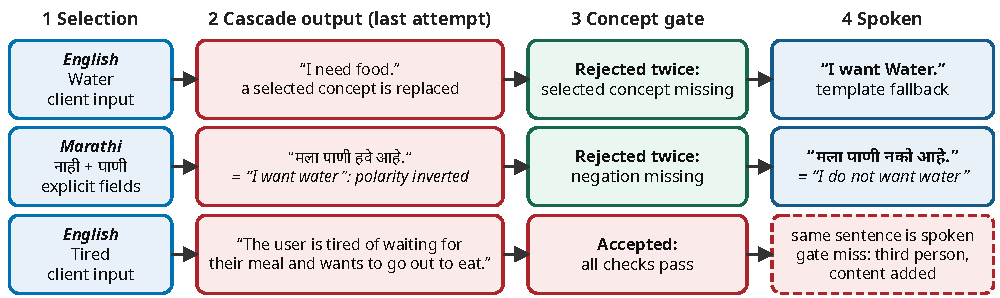
\includegraphics[width=\textwidth]{figures/teaser.pdf}
\caption{Three recorded scenarios from the frozen evaluation (rows 1 and 3: client input; row 2: explicit fields). The gate rejects a cascade output that replaces a selected concept (row~1) or inverts polarity (row~2), and the system then speaks a template fallback built from the user's labels; it accepts a fluent third-person sentence that adds content (row~3, a miss). Red: unwanted output or gate miss; green: correct gate decision; blue: selection or template fallback.}
\label{fig:teaser}
\end{figure*}


\begin{abstract}
Symbol-based augmentative and alternative communication (AAC) devices voice telegraphic labels, whereas Hindi, Gujarati, and Marathi sentences need case marking, agreement, and negation.
A language model can expand a selection into a sentence, but it can also replace a concept, drop a negation, or add content, and an AAC device speaks for its user.
We present \sys{}, a web system for English, Hindi, Gujarati, and Marathi that speaks a model-generated sentence only if a deterministic gate finds every selected concept and a matching negation (and, for English, checks the act and unrequested content), and otherwise speaks a template built from the user's own labels.
On \NPrimAll{} frozen scenarios sent as the web client builds them, the gate and its template fallback raised success from \XPreUSuccPct{} to \XDepUSuccPct{} and kept all \NConc{} required concept instances (the ungated cascade kept \XPreUKept{}) with no scored polarity error; with explicit intent fields, success rose from \XPreSSuccPct{} to \XDepSSuccPct{}.
The gate still admitted 59 of 110 failing cascade outputs, and a template baseline reached \XTmplUSuccPct{} and \XTmplSSuccPct{}, so under a lexical scorer the gate is a safeguard, not a quality gain.
The failure audit produced a repaired build, scored here only as a regression check.
A suffix-trie predictor exceeded a backoff trigram by 1.1 hit@1 points in English and 1.2 in Hindi on synthetic dialogues.
Speech synthesis is integrated but unverified, as no speech was produced; code, scenarios, and a screencast are at \demourl{}.
\end{abstract}

\section{Introduction}
\label{sec:intro}

A person who communicates through a symbol-based AAC board composes a message by tapping pictograms, and the device voices the selected labels.
The message is telegraphic (\emph{Water}, or \emph{No}\,+\,\emph{Pizza}), and the listener cannot see the selection, so a fluent sentence that misstates it can cause harm when the message is a request, a refusal, or a report of pain.
For a water request, a single \emph{Water} symbol can be realized as a complete sentence in each language (authored examples), with a verb-final, experiencer-dative construction for wanting:

\begin{center}
\small\renewcommand{\arraystretch}{1.12}
\begin{tabular}{@{}lll@{}}
\lang{Hindi} & \hi{मुझे पानी चाहिए।} & \multirow{3}{*}{\gloss{I want water.}}\\
\lang{Gujarati} & \gu{મને પાણી જોઈએ છે.} & \\
\lang{Marathi} & \hi{मला पाणी हवे आहे.} & \\
\end{tabular}
\end{center}

Feelings and negation use other constructions, so a literal join of labels is hard to parse.
A language model can generalize across combinations, but the small model that fits a 4\,GB GPU in our setup, \qwen{} \citep{qwen2025qwen25}, produced a successful sentence for only \XNaiveSucc{} scenarios when prompted without constraints (Section~\ref{sec:eval}).
Fluent output can still fail in three ways (Figure~\ref{fig:teaser}): the cascade evaluated here replaced the concept for \emph{Water}, inverted polarity for Marathi \emph{No}\,+\,\emph{Water}, and added content for \emph{Tired}.

\sys{} checks each candidate sentence against the selection.
A \emph{concept ledger} lists the concepts that must appear and those that must not, and a prompted cascade proposes a sentence.
A deterministic \emph{gate} accepts it only if its tests of concepts, negation, and communicative act pass; otherwise the system speaks a template fallback built from the user's own labels (Figure~\ref{fig:teaser}).
Among the closest systems (Section~\ref{sec:related}), none documents such a check for Indic symbol-to-speech, a setting relevant to symbol-board users and to the caregivers and clinicians who would configure boards.
\qwen{} and \indicf{} are used as released; our contributions are (i) the ledger, gate, and template fallback, with an interface that can carry intent explicitly (Section~\ref{sec:system}); (ii) a four-language demo with English and Hindi predictors trained on synthetic AAC dialogues (Section~\ref{sec:system}, Appendix Table~\ref{tab:models}); and (iii) a frozen, paired evaluation of \NPrimAll{} scenarios, an audit of what the gate misses, and the repair it led to (Sections~\ref{sec:eval} and~\ref{sec:repair}).

\section{Related Work}
\label{sec:related}

\paragraph{Expanding telegraphic input.}
Compansion expanded telegraphic AAC input into well-formed sentences \citep{mccoy1998compansion}.
Recent systems apply language models to other inputs. SpeakFaster expands abbreviated text for eye-gaze typists \citep{cai2024speakfaster}; ConnecTone suggests text from conversational context and speaks it with a style-adaptive text-to-speech (TTS) system \citep{francis2024connectone}; \citet{mohan2024composition} compose messages from typed, emoji, or spoken input in the user's own voice.
\citet{karmakar-sinha-2024-aiding} contribute a symbol-to-text dataset, a text-to-pictogram module, and an extension to Bengali, and \citet{francis2025static} add generated symbols and zero-shot voice cloning to a symbol board.
Constraining generated text to required content is established in lexically constrained decoding \citep{hokamp-liu-2017-lexically,post-vilar-2018-fast}.
\sys{} starts from symbol selections, which give the model a small concept set whose omission or inversion can be checked after generation, with a safe fallback; its novelty lies in that check and its evaluation, not in the expansion itself.

\paragraph{Gap.}
Table~\ref{tab:related} compares documented capabilities, including the boards Cboard, Jellow, and Avaz (\nstated{}: not stated by the source, not absent).
Among these sources, none documents a deterministic check of selected concepts and polarity in model-generated Indic sentences on a symbol board; we make no claim about undocumented products.

\begin{table*}[t]
\centering\footnotesize
\setlength{\tabcolsep}{3.6pt}\renewcommand{\arraystretch}{1.1}
\begin{tabular}{@{}L{3.6cm}L{2.5cm}L{3.5cm}L{2.7cm}L{2.4cm}@{}}
\toprule
\rowcolor{headtint}
System & Input & Languages (as stated) & Sentence realization & Output check \\
\midrule
Compansion \citeyearpar{mccoy1998compansion} & telegraphic words & English & grammatical expansion & \nstated \\
\citet{karmakar-sinha-2024-aiding} & symbols, text & incl.\ Bengali & symbol-to-text data & \nstated \\
Cboard \citeyearpar{cboard} & symbols, text & 46; HI, GU, MR not named & \nstated & \nstated \\
Jellow \citeyearpar{jellow} & symbols, keyboard & 24, incl.\ HI, GU, MR & pre-made, typed & \nstated \\
Avaz \citeyearpar{avaz} & symbols, keyboard & regional; list \nstated & predictive text & \nstated \\
ConnecTone \citeyearpar{francis2024connectone} & speech, text & \nstated & context suggestions & \nstated \\
SpeakFaster \citeyearpar{cai2024speakfaster} & abbreviated text & \nstated & LLM expansion & \nstated \\
\midrule
\rowcolor{rowtint}\textbf{\sys{}} & symbols, text & EN, HI, GU, MR & prompted \llm{Qwen} cascade & concepts, negation (act: EN) \\
\bottomrule
\end{tabular}
\caption{Documented capabilities of the closest systems, from the cited paper or the vendor page (access dates in the references). \nstated{}: not stated by the source; EN, HI, GU, MR: English, Hindi, Gujarati, Marathi.}
\label{tab:related}
\end{table*}

\section{System Design and Demo Walkthrough}
\label{sec:system}

\begin{figure*}[t]
\centering
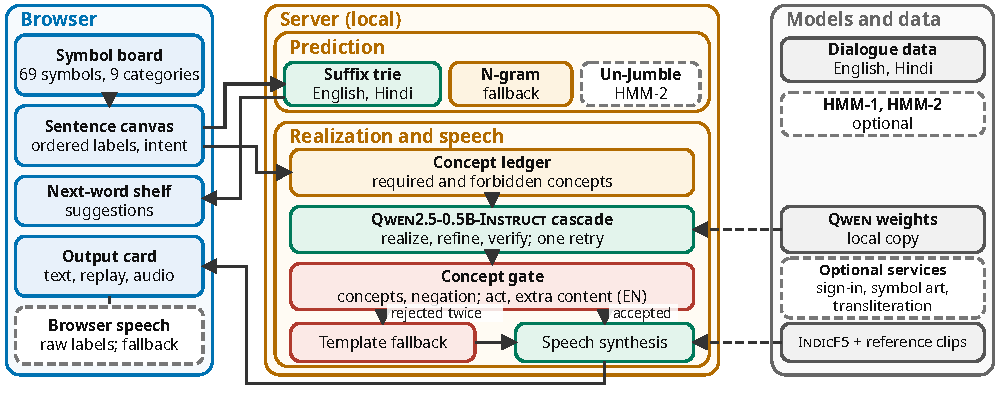
\includegraphics[width=0.92\textwidth]{figures/architecture.pdf}
\caption{Architecture of \sys{}; dashed boxes are optional. The cascade output is spoken only if the gate accepts it, and a template fallback is spoken after two rejections.}
\label{fig:arch}
\end{figure*}

\paragraph{Walkthrough.}
Figure~\ref{fig:arch} shows the decision path from a selection to the spoken sentence.
The user picks a language and taps symbols from a board of \NSymbols{} symbols in \NCategories{} categories, labeled in English, Hindi, Gujarati, and Marathi (Figure~\ref{fig:ui}, \cn{1}).
Selections accumulate on a sentence canvas (\cn{2}), and a shelf proposes next words with their probabilities (\cn{3}).
\emph{Speak} voices the literal labels with the browser's speech synthesis; \emph{AI Polish \& Speak} (\cn{4}) sends the selection to the server, which returns a sentence that the output card shows while it is spoken (\cn{5}).
\emph{Quick Express} speaks emergency phrases in one tap, and \emph{Un-Jumble} reorders canvas words with a second hidden Markov model (HMM).

\begin{figure}[t]
\centering
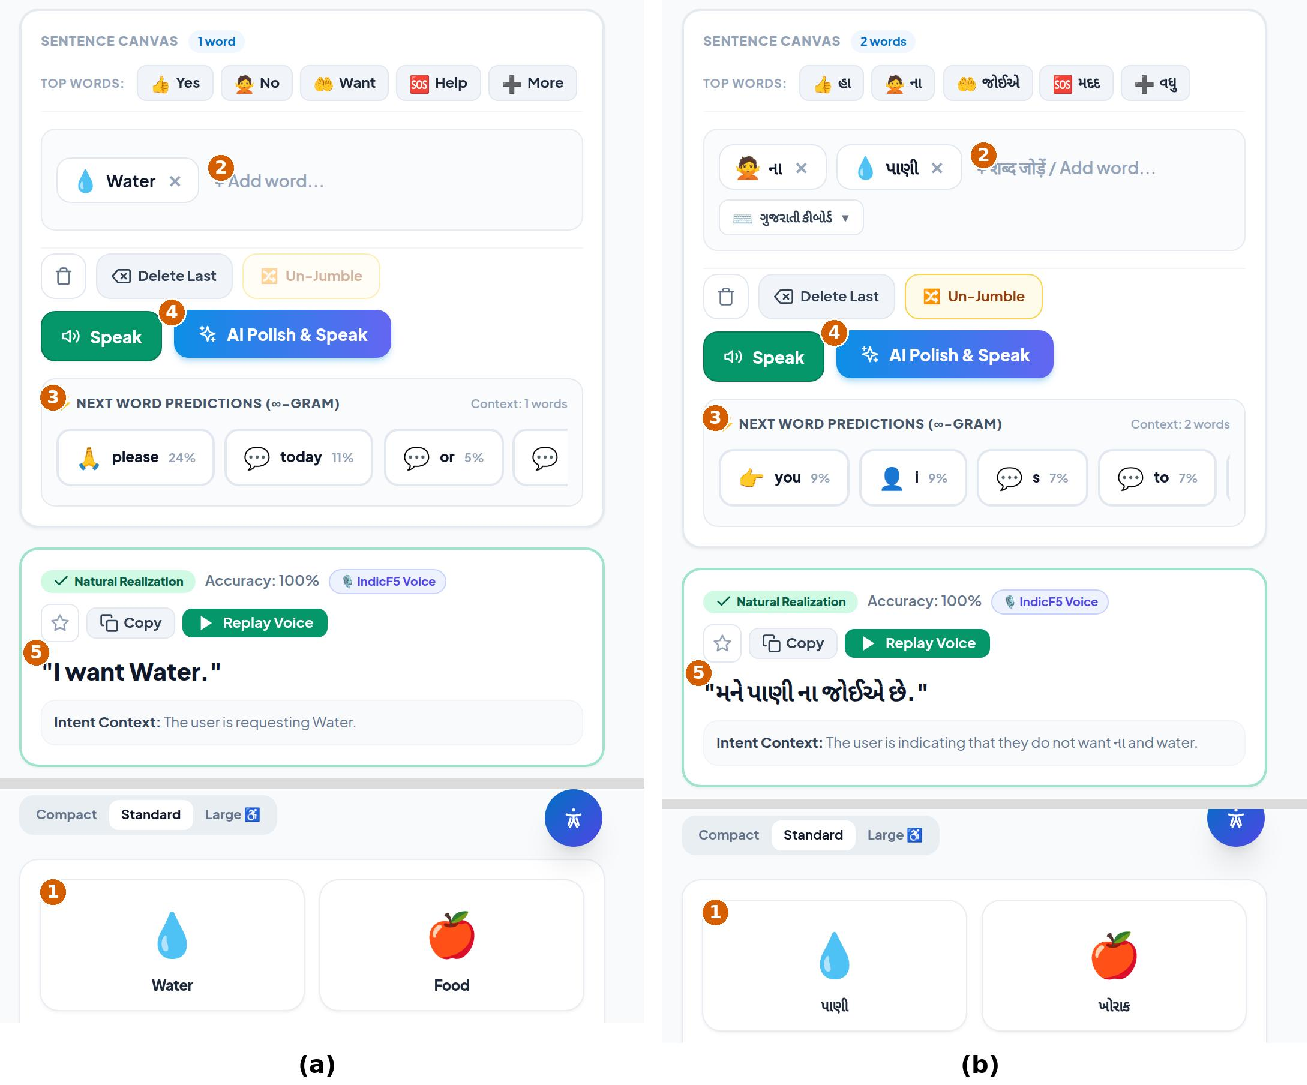
\includegraphics[width=0.9\columnwidth]{figures/ui_panel.pdf}
\caption{The evaluated build (the repaired build adds route chips, a message-type control, and a clarification card; Section~\ref{sec:repair}). (a)~English \emph{Water}: cascade output rejected, template fallback spoken. (b)~Gujarati \gu{ના}\,+\,\gu{પાણી}: cascade output accepted. The voice chip reads ``IndicF5 Voice'' although the server returned a placeholder tone; the \emph{Accuracy} badge is not used by the gate.}
\label{fig:ui}
\end{figure}

\paragraph{Input and concept ledger.}
The browser sends the ordered labels with the communicative intent (request, statement, question, or negation), a negation indicator, the language, and an optional code-mixing indicator.
The evaluated client infers intent and negation from label substrings (a negator in a label means negation, question words a question, a few feeling labels a statement, anything else a request); any other client can supply both fields explicitly, the explicit condition of Section~\ref{sec:eval}.
The server builds the ledger: a required set (intent, speaker, each selected concept, negation) and a forbidden set of 21 default words for unrequested times, meals, and venues, minus any word the user selected.

\paragraph{Realization and gate.}
Three prompted stages share one frozen \qwen{}.
The realizer writes a sentence from a few-shot prompt for Hindi, Gujarati, and Marathi (12, 9, and 9 examples; greedy decoding) and from a ledger prompt for English and code-mixed output (temperature 0.1).
The refiner removes unsupported content and is skipped for Indic-script candidates; the verifier returns a verdict, which is unused, and a minimal rewrite, which changed English candidates but no Indic one.
The gate decides by Equation~\eqref{eq:gate}, with $\nu$ the negation indicator, $E$ the selected concepts, $F$ the forbidden set, and $y$ the candidate:
\begin{equation}
\begin{split}
\mathrm{acc}(y)={}&[\mathrm{neg}(y)=\nu]\wedge\mathrm{match}(E,y)\wedge\mathrm{act}(y)\\
&\wedge\neg\mathrm{forbid}(y)\wedge\neg\mathrm{time}(y).
\end{split}
\label{eq:gate}
\end{equation}
Here \emph{neg} tests lists of English, Hindi, Gujarati, and Marathi negators; \emph{match} requires every selected concept to appear ; \emph{act} rejects ``I want'' for a feeling and requires a question cue for a question; \emph{forbid} matches a word of $F$; and \emph{time} flags time words when none was selected.
The act cues and the word lists are English only, so for Hindi, Gujarati, and Marathi the gate tests concept presence and negation.
A rejection triggers one more cascade run, and after two rejections a language-specific template fallback built from the selected labels (e.g., ``I want Water.'') is returned; English retries resample, whereas greedy Indic retries repeat the first output.

\paragraph{Prediction, speech, and training.}
Next-word suggestions come from an unbounded-order suffix trie in the spirit of infini-gram \citep{liu2024infinigram}, built at start-up from the English and Hindi AAC dialogues (\IGSent{} sentences, maximum depth \IGDepth{}).
Marathi reuses the Hindi trie and Gujarati has no predictor; two HMMs trained on streamed text (HMM-1 for next words, HMM-2 for Un-Jumble) are optional and were absent from the evaluated build.
The returned sentence is synthesized by \indicf{} \citep{ai4bharat2025indicf5}, a flow-matching model of the F5-TTS family \citep{chen2025f5tts}, with a 24\,kHz \vocos{} vocoder \citep{siuzdak2023vocos}, conditioned zero-shot on a reference clip and its transcript; the default clip is a Punjabi recording sent for every language, and an English narrator clip can be selected.
The model card lists Hindi, Gujarati, and Marathi but not English, so English speech is unverified.
Browser speech voices the literal labels and replaces server audio only when none is returned (Appendix~\ref{app:coverage}).
In the evaluated build no route produced speech: the gated weights were absent, so the server returned a placeholder tone that the client played, and headless Chrome exposed no voices.
We train the suffix trie, four HMMs, and an English \flant{} refiner (Appendix Table~\ref{tab:models}).

\section{Evaluation}
\label{sec:eval}

Realization is scored on \NPrimAll{} frozen scenarios (Tables~\ref{tab:results} and~\ref{tab:analysis}), next-word prediction on held-out conversations (Table~\ref{tab:pred}).

\paragraph{Protocol.}
We froze \NScen{} monolingual and \NScenCM{} exploratory Hinglish scenarios before scoring any output.
Each of English, Hindi, Gujarati, and Marathi has 46 board selections in six families (Appendix Table~\ref{tab:grid}), with gold polarity and act fixed.
Each scenario is sent as the web client builds it (\emph{client input}, the primary condition, because it is what a user's taps produce; the harness inputs equal those captured from the real page for all 184 scenarios) and with explicit intent and negation fields (\emph{explicit fields}, a controlled diagnostic of the cost of inferring intent, not a measure of user-selected intent).

\paragraph{Systems and scoring.}
We compare (i) a literal join of the labels; (ii) the same \qwen{} with one unconstrained zero-shot prompt (labels only); (iii) the ungated cascade, from the same response as the deployed output; (iv) the deployed output of the live server; and (v) the template baseline.
A scenario \emph{succeeds} if the output keeps every selected concept, has the gold polarity and act, adds no unselected concept, and is a first-person sentence in the target script; \emph{retention} counts the \NConc{} required concept instances separately.
A lexical scorer coded separately from the gate by the same team applies these rules (Appendix~\ref{app:scorer}); all counts here use its first version, and Section~\ref{sec:repair} reports its correction.
Nine of the \NScen{} scenarios, which duplicate a few-shot prompt example, are excluded, leaving \NPrimAll{} (EN \NPrimEN{}, HI \NPrimHI{}, GU \NPrimGU{}, MR \NPrimMR{}).
Differences (in percentage points, pp) are paired, with 95\% bootstrap confidence intervals (CI) over the 46 scenario groups (the four language versions of one board selection; 10,000 resamples).

\begin{table*}[t]
\centering\footnotesize
\setlength{\tabcolsep}{3.2pt}
\begin{tabular}{@{}l ccccc @{\hspace{6pt}} c ccccc@{}}
\toprule
 & \multicolumn{5}{c}{Scenario success (n/N)} & \multicolumn{6}{c}{Pooled diagnostics (counts)} \\
\cmidrule(lr){2-6}\cmidrule(l){7-12}
System & EN & HI & GU & MR & All & Kept$\uparrow$ & Pol.$\downarrow$ & \shortstack{Wrong\\act$\downarrow$} & \shortstack{No\\act$\downarrow$} & Added$\downarrow$ & \shortstack{Off-\\task$\downarrow$} \\
\midrule
\multicolumn{12}{@{}l}{\emph{Client input (intent and negation inferred from the labels)}}\\
Unconstrained \llm{Qwen} & 2/46 & 1/45 & 4/42 & 1/42 & 8/175 & 199/215 & 2 & 3 & 163 & 7 & 16 \\
Ungated cascade & 3/46 & 24/45 & 20/42 & 18/42 & 65/175 & 175/215 & 2 & 54 & 33 & 25 & 19 \\
\rowcolor{rowtint}\textbf{\sys{} (deployed)} & \textbf{22/46} & \textbf{31/45} & \textbf{21/42} & \textbf{23/42} & \textbf{97/175} & \textbf{215/215} & \textbf{0} & \textbf{54} & \textbf{21} & \textbf{4} & \textbf{10} \\
Template baseline & 33/46 & 31/45 & 27/42 & 27/42 & 118/175 & 215/215 & 0 & 57 & 0 & 0 & 0 \\
\midrule
\multicolumn{12}{@{}l}{\emph{Explicit fields (gold intent and negation supplied)}}\\
Ungated cascade & 5/46 & 26/45 & 16/42 & 24/42 & 71/175 & 185/215 & 36 & 30 & 44 & 21 & 17 \\
\rowcolor{rowtint}\textbf{\sys{} (deployed)} & \textbf{33/46} & \textbf{41/45} & \textbf{26/42} & \textbf{32/42} & \textbf{132/175} & \textbf{215/215} & \textbf{0} & \textbf{17} & \textbf{24} & \textbf{3} & \textbf{9} \\
Template baseline & 46/46 & 45/45 & 34/42 & 42/42 & 167/175 & 215/215 & 0 & 0 & 8 & 0 & 0 \\
\bottomrule
\end{tabular}
\caption{Primary set (175 scenarios; EN 46, HI 45, GU 42, MR 42), scorer version 1. Kept: required concept instances present (of 215). Pol. to Off-task: scenarios (of 175) with that error (one output can have several); off-task is defined in Appendix~\ref{app:scorer}. A literal join succeeds on 0/175 scenarios (no act marker) and keeps 215/215 concepts.}
\label{tab:results}
\end{table*}

\begin{table}[t]
\centering\footnotesize
\setlength{\tabcolsep}{3pt}
\begin{tabular}{@{}lcccccc@{}}
\toprule
 & \multicolumn{3}{c}{English} & \multicolumn{3}{c}{Hindi} \\
\cmidrule(lr){2-4}\cmidrule(l){5-7}
Model & @1 & @5 & MRR & @1 & @5 & MRR \\
\midrule
Unigram frequency & 3.6 & 11.6 & 0.069 & 6.4 & 14.5 & 0.099 \\
Bigram, backoff & 13.6 & 29.5 & 0.204 & 24.0 & 43.1 & 0.320 \\
Trigram, backoff & 16.0 & 32.8 & 0.234 & 25.9 & 44.0 & 0.334 \\
Gutenberg HMM & 6.7 & 15.5 & 0.105 & -- & -- & -- \\
Hindi AAC HMM & -- & -- & -- & 24.5 & 41.9 & 0.315 \\
\midrule
\rowcolor{rowtint}\textbf{$\infty$-gram (deployed)} & \textbf{17.2} & \textbf{33.4} & \textbf{0.240} & \textbf{27.0} & \textbf{44.1} & \textbf{0.343} \\
\bottomrule
\end{tabular}
\caption{Next-word prediction on AAC-user turns of synthetic dialogues (LLM-generated English, machine-translated Hindi): 60 of the 300 source conversations per language are held out (240 train), giving 2,220 English and 2,437 Hindi contexts; hit rates (@1, @5) in \%; MRR: mean reciprocal rank over the top 10. Text differences are computed from counts. Held-out sources share 18 of 392 English and 28 of 384 Hindi distinct utterances with training; \PredOOVEN{} (EN) and \PredOOVHI{} (HI) of targets are out of vocabulary and count as misses. Gujarati and Marathi are not evaluated: the 34-language collection of \citet{vertanen2026multilingual} has neither, and we know of no other AAC corpus for them.}
\label{tab:pred}
\end{table}


\paragraph{Effect of the gate.}
Before the gate, the cascade kept \XPreUKeptPct{} of required concepts under client input (\XPreSKeptPct{} with explicit fields) and made \XPreUPol{} polarity errors, against \XPreSPol{} with explicit fields, whose inputs do not carry the \emph{No} label as an entity (Table~\ref{tab:results}).
With the gate and template fallback, the same scenarios kept all \NConc{} concepts and showed no scored polarity error; the scorer, like the gate, tests for a negator and not its scope, so these counts are not a guarantee of meaning.
Success rose from \XPreUSucc{} to \XDepUSucc{} under client input (+18.3 pp, 95\% CI 11.9 to 25.2) and from \XPreSSucc{} to \XDepSSucc{} with explicit fields (+34.9, 26.7 to 43.4).
All 33 scenarios that the gate turned from failure into success under client input are template sentences, 20 of them English, and for Hindi, Gujarati, and Marathi alone the gain is +10.1 pp (5.2 to 16.0).
Under client input the gate accepted \XGateAccU{} model outputs (\XGateOkU{} fully correct), admitted 59 of the 110 failing cascade outputs, and its template fallbacks succeeded in \XFbOkU{} (explicit fields: \XGateOkS{} and \XFbOkS{}; Appendix~\ref{app:scorer} audits the failures).
The first cascade stage alone scores 63/175 and 67/175, against 65/175 and 71/175 for the full cascade.

\paragraph{Remaining errors.}
Under client input, \XDepUWrong{} deployed outputs expressed the wrong act; explicit fields cut this to \XDepSWrong{} and raised success from \XDepUSuccPct{} to \XDepSSuccPct{} (+20.0 pp, 12.0 to 28.7).
The client infers \emph{request} for \UIFeelReq{} of its 32 single-symbol feeling selections (eight feelings in four languages, before the nine exclusions), so every language voices a feeling as a want (Table~\ref{tab:analysis}), and the gate does not catch it, because its act test uses English cues.
Two defects are independent of the model: the client's substring rule wrongly marks \UIFalseNeg{} of 272 non-negated single-symbol selections as negated (\emph{Nose} in English and Gujarati, \emph{Bathe} in Gujarati), and the template has no form for client intent \emph{negation} (negated feeling, Appendix Table~\ref{tab:grid}).
Accepted outputs can also add content or a third-person perspective (Figure~\ref{fig:teaser}, row~3; Appendix Figure~\ref{fig:workflow} and Tables~\ref{tab:grid} and~\ref{tab:kinds}).

\begin{table*}[t]
\centering\footnotesize
\setlength{\tabcolsep}{3.4pt}\renewcommand{\arraystretch}{1.2}
\begin{tabular}{@{}L{2.35cm}L{2.95cm}L{3.0cm}L{3.1cm}L{3.1cm}@{}}
\toprule
\rowcolor{headtint}
Selection $\rightarrow$ intended & \lang{English} (baseline) & \lang{Hindi} & \lang{Gujarati} & \lang{Marathi} \\
\midrule
\emph{Angry} $\rightarrow$ \gloss{I am angry}
 & \bad{I want} \sel{Angry.} \routet\ \failmark{W}
 & \hi{\bad{मुझे} \sel{गुस्सा} \bad{चाहिए।}} \routem\ \failmark{W}
 & \gu{\bad{મને} \sel{ગુસ્સો} \bad{જોઈએ છે.}} \routem\ \failmark{W}
 & \hi{\bad{मला} \sel{रागात} \bad{हवे आहे.}} \routem\ \failmark{W} \\
\bottomrule
\end{tabular}
\caption{One selection in four languages, deployed output with client input (recorded). \sel{Blue}: selected concept kept; \kept{green}: passes the scorer; \bad{red}: unwanted act or added content; \okmark{} success; \failmark{W} wrong act, \failmark{N} no act marker, \failmark{A} added content; \routem{} accepted model output, \routet{} template fallback. English is the baseline; the Indic columns are the proposed extension.}
\label{tab:analysis}
\end{table*}

\paragraph{Template baseline.}
A template baseline echoes the selected labels, so it scored \XTmplSSucc{} with explicit fields and \XTmplUSucc{} under client input; the deployed pipeline trailed it by 20.0 pp (95\% CI 14.0 to 26.4) and 12.0 pp (6.4 to 17.9).
Paired by scenario, the pipeline succeeded where the template failed in 0 of 175 scenarios (explicit fields) and 1 (client input), and failed where it succeeded in 35 and 22.
Matching the eight explicit-field template failures to their scenarios places all of them in Gujarati negated feelings.
The template sentence \gu{મને ખુશ લાગતું નથી.} was missing from the scorer's marker list, whereas its Hindi and Marathi counterparts (\hi{मुझे खुश महसूस नहीं हो रहा है।} and \hi{मला आनंदी वाटत नाही.}) were recognized (all three: \gloss{I do not feel happy}); we read these failures as scorer gaps, but no native speaker has checked the sentences.
The model path added wrong-act outputs that a template did not (\XDepSWrong{} against \XTmplSWrong{}), and the lexical criterion rewards label echo without scoring fluency, so the comparison cannot measure what model phrasing adds.

\paragraph{Next-word prediction.}
The suffix trie exceeded unigram and bigram baselines in both languages and a backoff trigram by \PredDENOneTri{} hit@1 in English (381 against 356 of 2,220 contexts) and \PredDHIOneTri{} in Hindi (659 against 630 of 2,437), computed from counts with a paired bootstrap over source conversations (Table~\ref{tab:pred}).

\section{Failure Audit and Repairs}
\label{sec:repair}

The audit traced the errors above to defects in four components, each repaired, with the build frozen by recorded file hashes before any new scenario was drawn.
\textbf{Interface:} concept identifiers on board symbols, separate act and polarity fields, whole-token matching of typed words, and a message-type control with a two-button clarification card; tested on the real page, the evaluated client sent a wrong act for 59 of 184 scenarios and the repaired client for none.
\textbf{Gate and templates:} the gate tests the writing system, speaker perspective, concept presence with inflected forms, added content, clause-scoped negation, and the act marker, with a stated reason per rejection; compositional templates cover requests, refusals, feelings, negated feelings, actions, and calls for help, and an uncovered selection yields a labeled literal preview.
\textbf{Scorer:} version 2 adds valid constructions that version 1 missed and scopes negation to its clause; the deployed count moves from 97 to 95 (client input; 5 scenarios gained, 7 lost) and from 132 to 138 (explicit fields), the ungated cascade from 65 to 63 and from 71 to 72, and the template baseline from 167 to 175, which widens the gaps to the template to 13.1 and 21.1 pp.

\paragraph{Regression result.}
On the original \NPrimAll{} scenarios under version 2, the repaired pipeline and the repaired template baseline both score 175/175 (the repaired client sends the gold fields, so client input and explicit fields coincide), against 95 and 138 for the evaluated build and 8/175 for a new one-pass prompt with the repaired fields; the repaired pipeline exceeds the same cascade without gate and fallback (88/175) by 49.7 pp (95\% CI 42.3 to 57.1).
These scenarios informed the repairs, so 175/175 is a regression target and not a test result, and a lexical scorer cannot separate pipeline from template.
A fresh set of 120 scenarios (30 per language) generated after the freeze awaits native-speaker confirmation of its gold annotation, so no score on it is reported.

\section{Availability, License, and Limitations}
\label{sec:limits}

\paragraph{Availability and license.}
The reviewer package (source, frozen scenarios, scorer, raw outputs, installation guide) and a two-minute captioned screencast without audio are at \demourl{}.
Code is released under the \codelicense{}; models and fonts keep their own licenses (Appendix Table~\ref{tab:models}); installation tests are in Appendix~\ref{app:coverage}.

\paragraph{Limitations.}
The scorer is lexical and its Indic lexicon is not native-reviewed; scenarios cover one- and two-concept selections from a \NSymbols{}-symbol board; one team wrote the rules, gold annotation, and scorer, with AI assistance and without an independent curator.
No user study has been run, so the results bound lexical faithfulness, not communication effectiveness.
Speech was a placeholder tone, so latency (Appendix~\ref{app:coverage}) excludes synthesis, and \indicf{} speech quality was not assessed (Appendix Table~\ref{tab:mos} scores the tone and stand-in voices only).
Gujarati has no predictor and Marathi reuses the Hindi trie; extending Table~\ref{tab:pred} to both needs AAC dialogue corpora.
In the evaluated build the template fallback is not re-validated, and the gate's act test and word lists cover English only.

\section{Conclusion}
\label{sec:conclusion}

Across \NPrimAll{} frozen scenarios in four languages, deterministic checks kept every selected concept and left no scored polarity error, but only 57 of the 116 sentences accepted under client input were fully correct, and a template baseline matched or exceeded the pipeline under a lexical scorer.
Native-speaker confirmation of a fresh scenario set, blind ratings of meaning and phrasing, and audible speech in all four languages are the next steps toward measuring what model phrasing adds.


\section*{Ethics Statement}
An AAC device speaks for a person, so a plausible but wrong sentence can misstate consent or refusal.
The gate lowers this risk without removing it: it checks selected concepts, polarity, and a limited set of act cues, not meaning in full.
The evaluated interface speaks a sentence as soon as it is ready and does not show when a template replaced model output; the repaired build labels templates and does not speak a clarification or a literal preview unprompted, but consequential messages should still be confirmed with the user or a caregiver, and a preview-and-confirm step for generated sentences is a priority for deployments.
Direct \emph{Speak} and Quick Express remain available when generated text is unsuitable.

Voice cloning requires a reference clip and its exact transcript from the speaker or a guardian, with consent; clones are held in server memory only.
Optional features can send typed words to third parties (Google Input Tools, OpenAI Images) or store My Words and bookmarks in Firebase; generation, prediction, and speech do not need them.
The evaluation uses synthetic dialogues and scripted scenarios and contains no personal data; a study with AAC users would need accessible consent and the option to withdraw data.
Accessibility testing covered keyboard activation, emulated touch, and automated checks of names and live regions, not screen readers or switch scanning; the page has no live region for new text and renders nothing when the content delivery networks that serve its React, Babel, and Tailwind libraries are blocked, although generation and prediction run on the local server.
Cloning can also impersonate a person, so the consent requirement above must be kept.
Quality differs across languages: model output is weakest in English, the Indic output rests on few-shot prompts, and no native speaker has reviewed the Indic sentences, so Gujarati and Marathi deployments need that review first.
Hindi and Marathi first-person sentences can mark the speaker's gender; the repaired templates avoid it where a neutral construction exists, but model output may not.
The HMM-1 and HMM-2 checkpoints were absent from the evaluated build, so HMM-1 prediction and Un-Jumble are not evaluated.


\section*{Acknowledgements}
We used generative AI assistants (Claude by Anthropic; ChatGPT and Codex by OpenAI) to merge two snapshots of the system into the version evaluated here; to write the evaluation harness, scorer lexicon, scenario gold annotations, and failure classification; to generate the figure scripts and check references; to repair the interface, gate, and templates described in Section~\ref{sec:repair}; and to draft and edit this paper.
No native speaker has reviewed the lexicon, the gold annotations, or the templates.
All reported numbers were checked against the recorded result files.
The AAC dialogue data were generated with OpenAI \llm{gpt-4o-mini}, and the Hindi dialogues are machine translations (\llm{opus-mt-en-hi}).


\bibliography{references}

\clearpage
\appendix
\twocolumn[{%
\makeatletter
\section{Interaction Trace and Test Cases}\label{app:trace}\label{app:tests}
\centering
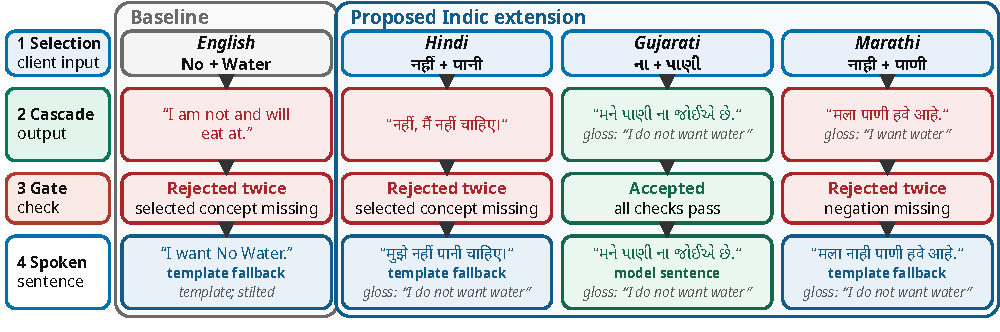
\includegraphics[width=\textwidth]{figures/fig4_languages.pdf}
\captionof{figure}{One selection (\emph{No}\,+\,\emph{Water}) in four languages (recorded outputs, client input). Red: rejected cascade output; blue: template fallback; green: accepted model sentence; italics: the authors' gloss. The word order of the template sentences is not native-reviewed.}
\label{fig:workflow}
\vspace{2pt}
\centering\footnotesize
\setlength{\tabcolsep}{3.2pt}\renewcommand{\arraystretch}{1.02}
\begin{tabular}{@{}L{2.5cm}L{2.95cm}L{2.85cm}L{3.0cm}L{3.0cm}@{}}
\toprule
\rowcolor{headtint}
Family ($n$): selection & \lang{English} (baseline) & \lang{Hindi} & \lang{Gujarati} & \lang{Marathi} \\
\midrule
Request (35): \emph{Fruit}
 & \kept{I want Fruit.} \routet\ \okmark
 & \hi{\kept{मुझे फल चाहिए।}} \routem\ \okmark
 & \gu{\kept{મને ફળ જોઈએ છે.}} \routem\ \okmark
 & \hi{\kept{मला फळ हवे आहे.}} \routem\ \okmark \\
\rowcolor{rowtint}
Refusal (38): \emph{No}\,+\,\emph{Fruit}
 & \bad{I am not a} \sel{fruit}\bad{. I do not eat fruits.} \routem\ \failmark{W,A}
 & \hi{\kept{फल नहीं है, नहीं चाहिए।}} \routem\ \okmark
 & \gu{\sel{મારે ના ફળ છે.}} \routem\ \failmark{N}
 & \hi{\kept{मला नाही फळ हवे आहे.}} \routet\ \okmark \\
Feeling (30): \emph{Angry}
 & \bad{I want} \sel{Angry.} \routet\ \failmark{W}
 & \hi{\bad{मुझे} \sel{गुस्सा} \bad{चाहिए।}} \routem\ \failmark{W}
 & \gu{\bad{મને} \sel{ગુસ્સો} \bad{જોઈએ છે.}} \routem\ \failmark{W}
 & \hi{\bad{मला} \sel{रागात} \bad{हवे आहे.}} \routem\ \failmark{W} \\
\rowcolor{rowtint}
Negated feeling (32): \emph{No}\,+\,\emph{Angry}
 & \bad{I want} \sel{No Angry.} \routet\ \failmark{W}
 & \hi{\sel{गुस्सा,} \bad{नहीं चाहिए।}} \routem\ \failmark{W}
 & \gu{\sel{મારે ના ગુસ્સો છે.}} \routem\ \failmark{N}
 & \hi{\bad{मला} \sel{नाही रागात} \bad{हवे आहे.}} \routet\ \failmark{W} \\
Action (24): \emph{Drink}\,+\,\emph{Milk}
 & \bad{The user requested} \sel{milk} \bad{for their drink.} \routem\ \failmark{N,P}
 & \hi{\kept{मुझे पीना दूध चाहिए।}} \routet\ \okmark
 & \gu{\kept{મને પીવું જોઈએ છે. દૂધ આપે.}} \routem\ \okmark
 & \hi{\kept{मला पिणे दूध हवे आहे.}} \routem\ \okmark \\
\rowcolor{rowtint}
Call (16): \emph{Call}\,+\,\emph{Doctor}
 & \kept{I want Call Doctor.} \routet\ \okmark
 & \hi{\kept{फ़ोन करना गया है, मुझे डॉक्टर चाहिए।}} \routem\ \okmark
 & \gu{\sel{મને ડૉક્ટર ફોન કરવો છે.}} \routem\ \failmark{N}
 & \hi{\sel{मला डॉक्टर फोन करणे मिळू शकता का?}} \routem\ \failmark{N} \\
\bottomrule
\end{tabular}
\captionof{table}{One scenario per family (the first alphabetical one present in all four languages), deployed output with client input (recorded). Intended messages: \gloss{I want fruit}, \gloss{I do not want fruit}, \gloss{I am angry}, \gloss{I am not angry}, \gloss{I want to drink milk}, \gloss{I want to call the doctor}. Colors, marks, and tags as in Table~\ref{tab:analysis}; \failmark{P}: third-person report. Green marks a scorer pass, not fluency (\emph{I want Call Doctor.}); no native speaker has judged these outcomes; the Gujarati and Marathi \emph{Call} outputs are a scorer gap and a question form.}
\label{tab:grid}
\makeatother
}]

\begin{table*}[!t]
\centering\footnotesize
\setlength{\tabcolsep}{3.2pt}\renewcommand{\arraystretch}{1.02}
\begin{tabular}{@{}L{2.9cm}L{2.3cm}L{5.2cm}L{5.1cm}@{}}
\toprule
\rowcolor{headtint}
Kind of outcome & Input & Recorded output & Result \\
\midrule
Unrequested content, caught & \lang{English}, client: \emph{No}\,+\,\emph{Water} & first candidate \bad{I am not hungry. I will eat at the restaurant.} & rejected: concept missing, and \emph{hungry} and \emph{restaurant} are forbidden words \\
\rowcolor{rowtint}Code-mixed input (exploratory) & \lang{Hinglish}, API input: \emph{Pizza} & \bad{The user requested a pizza.} \routem & accepted by the gate; fails scorer (third person, English for Hindi); the template baseline succeeds \\
Ambiguous selection; server unreachable (repaired client) & \lang{English}: \emph{Nose}; any language & card \gloss{What do you want to say?} with buttons \gloss{I want something} and \gloss{I feel something}; literal labels as a preview & nothing is spoken until the user chooses; nothing is guessed \\
\bottomrule
\end{tabular}
\caption{One recorded example of each further kind of outcome (colors and tags as in Table~\ref{tab:analysis}; Figure~\ref{fig:teaser} shows three more kinds). The last row shows demo states of the repaired build, not scored scenarios.}
\label{tab:kinds}
\end{table*}


\begin{table*}[!t]
\centering\footnotesize
\setlength{\tabcolsep}{3pt}\renewcommand{\arraystretch}{1.02}
\begin{tabular}{@{}L{4.0cm}L{8.1cm}L{3.4cm}@{}}
\toprule
\rowcolor{headtint}
Component and role & Training or adaptation & Data or license \\
\midrule
\qwen{}: realizer, refiner, verifier & Prompted, not fine-tuned (few-shot for HI, GU, MR); rev.\ 7ae5576 & Apache-2.0 \\
\indicf{} + \vocos{}: speech & Pretrained; zero-shot voice from a clip and its transcript & 1,417\,h; MIT, gated \\
HMM-1, HMM-2: optional next word, Un-Jumble & Streamed in 500K-sentence chunks, count-pruned; HMM-1: Jelinek--Mercer weights 0.50/0.30/0.15/0.05; HMM-2: word and part-of-speech trigrams, beam 64 & English sentences, Tatoeba, Pile slices \\
Gutenberg HMM, Hindi AAC HMM: baselines & Bigram and trigram counts over 188,402 sentences (713,845 trigram states); 3,867 Hindi turns (3,078 for evaluation) & public-domain books; Hindi dialogues \\
Suffix trie ($\infty$-gram): primary next word & Count-based, built at start-up (\IGSent{} sentences, depth \IGDepth{}) & English and Hindi dialogues \\
\flant{} refiner: companion tool & Fine-tuned (learning rate $10^{-4}$, batch 16 with two accumulation steps, 10 epochs, seed 42, one TITAN Xp, 204\,s) after a 500-update fluency adaptation on 4,380 denoising pairs; on 384 test inputs it reaches \RefAModel{} exact match (\RefFModel{} with the adaptation) and no negation error in 172 negated inputs; rules score \RefARules{} (references come from the same templates) & 3,052 template inputs (384 validation, 384 test) \\
\bottomrule
\end{tabular}
\caption{Learned components, from the training records and model files in the release package; \qwen{} and \indicf{} are used as released; Noto fonts: SIL OFL 1.1.}
\label{tab:models}
\end{table*}

\begin{table*}[!t]
\centering\footnotesize
\setlength{\tabcolsep}{3.4pt}\renewcommand{\arraystretch}{1.1}
\begin{tabular}{@{}l c ccc cccc c@{}}
\toprule
\rowcolor{headtint}
 & Evaluated build & \multicolumn{3}{c}{Human voice prompts} & \multicolumn{4}{c}{Stand-in voice, deployed sentences} & Deployed voice \\
\rowcolor{headtint}
 & \lang{Tone} (1) & \lang{English} (1) & \lang{Marathi} (3) & \lang{Punjabi} (1) & \lang{English} (46) & \lang{Hindi} (45) & \lang{Gujarati} (42) & \lang{Marathi} (42) & \indicf{} (0) \\
\midrule
\utmos{} & \bad{1.54} & 4.27 & 3.20 & 3.83 & 4.01 (0.31) & 3.66 (0.38) & 3.88 (0.24) & 3.31 (0.41) & not run \\
\rowcolor{rowtint}\nisqa{} & \bad{1.12} & 4.50 & 4.81 & 4.74 & 4.39 (0.61) & 3.52 (0.59) & 4.91 (0.10) & 3.95 (0.64) & not run \\
\bottomrule
\end{tabular}
\caption{Predicted speech quality (1--5, higher is better; mean, and standard deviation for the synthesized voices; clips in the header). \emph{Tone}: the evaluated build's placeholder. Human prompts: clips that \indicf{} would imitate (Punjabi: the default for all languages). Stand-in voices: open \mmstts{} models reading the deployed sentences, not \indicf{}, whose weights are gated. Both predictors are trained on English ratings (indicative only).}
\label{tab:mos}
\end{table*}


\section{Scorer, Failure Audit, Speech, and Runtime}
\label{app:scorer}\label{app:coverage}
Retention is the share of required concept instances present. Polarity is correct when a negator is present exactly if the gold message is negated (its scope is not checked), and the act is correct when a request marker (want, need, \hi{चाहिए}, \gu{જોઈએ}, \hi{हवे}) or, for feelings, a feeling marker without a request marker is present. A concept is \emph{added} if any other board concept or a time, meal, or venue word occurs.
An output is \emph{off-task} if it is a model refusal or meta-comment, is a third-person report (``the user\ldots''; English only), is empty or longer than 25 tokens, or contains Latin text in an Indic target; a user's own refusal is never off-task. With explicit fields, feelings carry the intent \textsc{statement} (chosen after an aborted 54-request pilot).
\emph{Failure audit.} Of the 37 accepted outputs that fail the scorer with explicit fields, 35 are genuine failures (12 negated want for a negated feeling, 10 ungrammatical, 9 third-person reports, 4 added content) and two are marker-list gaps, as are all six failing template fallbacks and all eight failing template-only outputs (AI-assisted classification, not native-checked).
Exploratory Hinglish (8 scenarios; client input, explicit fields): deployed \CMSuccDepU{}, \CMSuccDepS{}; unconstrained \CMSuccNaive{}; template baseline \CMSuccTmplU{}, \CMSuccTmplS{}.


Speech routes to \indicf{} with the default Punjabi reference clip for every language; browser voices (hi-IN, gu-IN, mr-IN, en-US; Gujarati and Marathi fall back to hi-IN, then en-IN) speak only when the server returns no audio. Neither route was verified: the gated weights were absent (placeholder tone) and the test browser exposed no voices. Table~\ref{tab:mos} scores the tone, the prompt clips, and, as a pipeline check only, the deployed sentences read by open \mmstts{} voices \citep{pratap2023mms}, with \utmos{} \citep{saeki2022utmos} and \nisqa{} \citep{mittag2021nisqa}; both are trained on English ratings, so the values are indicative and do not describe \indicf{}.
Gate-accepted requests took a median of \LatMedAccEN{}, \LatMedAccHI{}, \LatMedAccGU{}, and \LatMedAccMR{}\,s (EN, HI, GU, MR) and twice-rejected ones \LatFbMin{}--\LatFbMax{}\,s on the GTX~1650, against about 0.4\,ms for a repaired template on a CPU; the verifier takes a median of \StageLlmThree{}\,s per request and never changed the first-stage text of a Hindi, Gujarati, or Marathi scenario (129 of 129); on the repaired build, click to first playback of the placeholder tone took a median of 9.9\,s (31 warm runs), so time to audible speech is unmeasured.
A fresh CPU environment completed the documented request in 44\,s (no weight download or GPU installation tested), and generation and prediction also completed with downloads disabled and non-local connections refused.



\end{document}
